\PassOptionsToPackage{xcolor}{svgnames}
\documentclass[french]{beamer}
\usepackage{multimedia}
\usepackage[utf8]{inputenc}
\usepackage[T1]{fontenc}
\usepackage{babel}
\usepackage{hyperref}

\title{Modélisation \& Vérification de réseaux ferroviaires avec CosyVerif}
\subtitle{Ou comment tricher à Transport Tycoon...}
\begin{document}

\begin{frame}
\maketitle
\end{frame}

\begin{frame}
  \frametitle{Des réseaux ferroviaires (presque) réels}
  \begin{center}
  \href{http://www.openttd.org}{OpenTTD} : réimplémentation libre de Transport Tycoon Deluxe

  
\includegraphics[height=1em]{images/openttd-64.png}~~~~~\url{http://www.openttd.org}

  \bigskip
  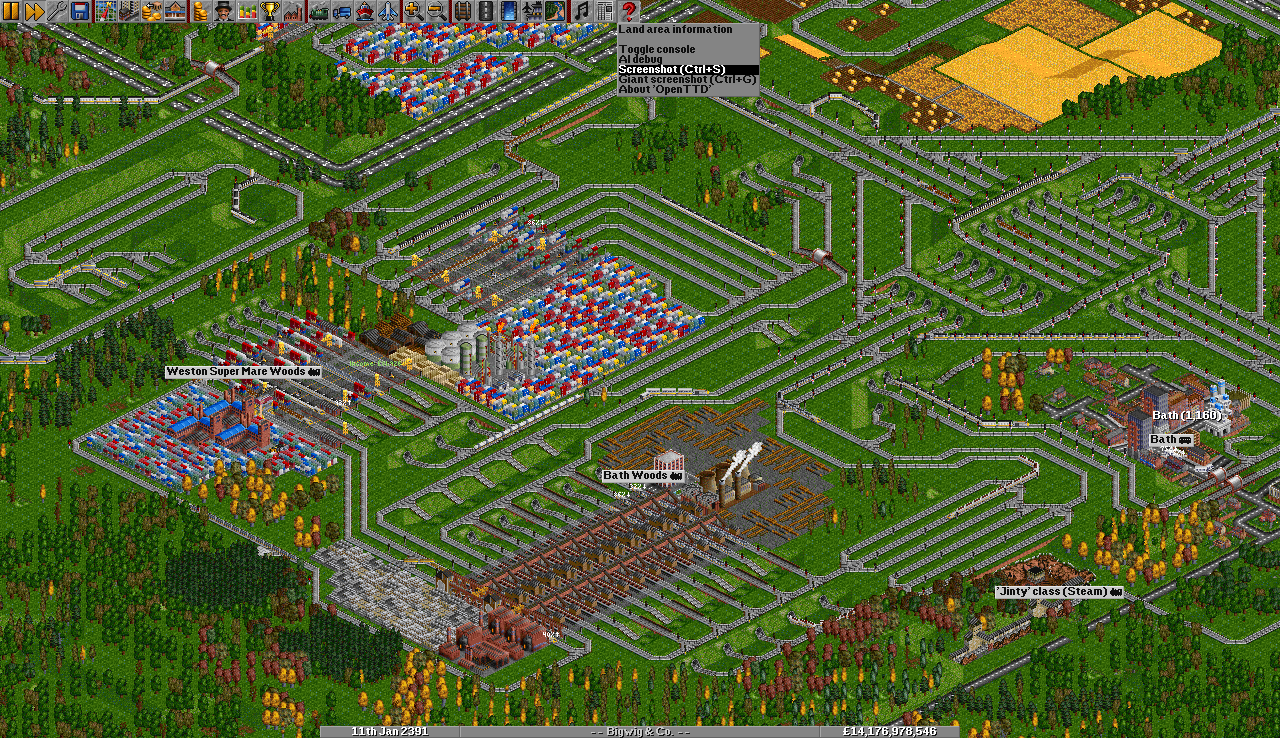
\includegraphics[width=.95\textwidth]{images/screen.png}  
  \end{center}
\end{frame}

\begin{frame}
  \frametitle{\href{http://cosyverif.org}{CosyVerif}
  un environnement de Modélisation \& Vérification}
  \begin{center}
  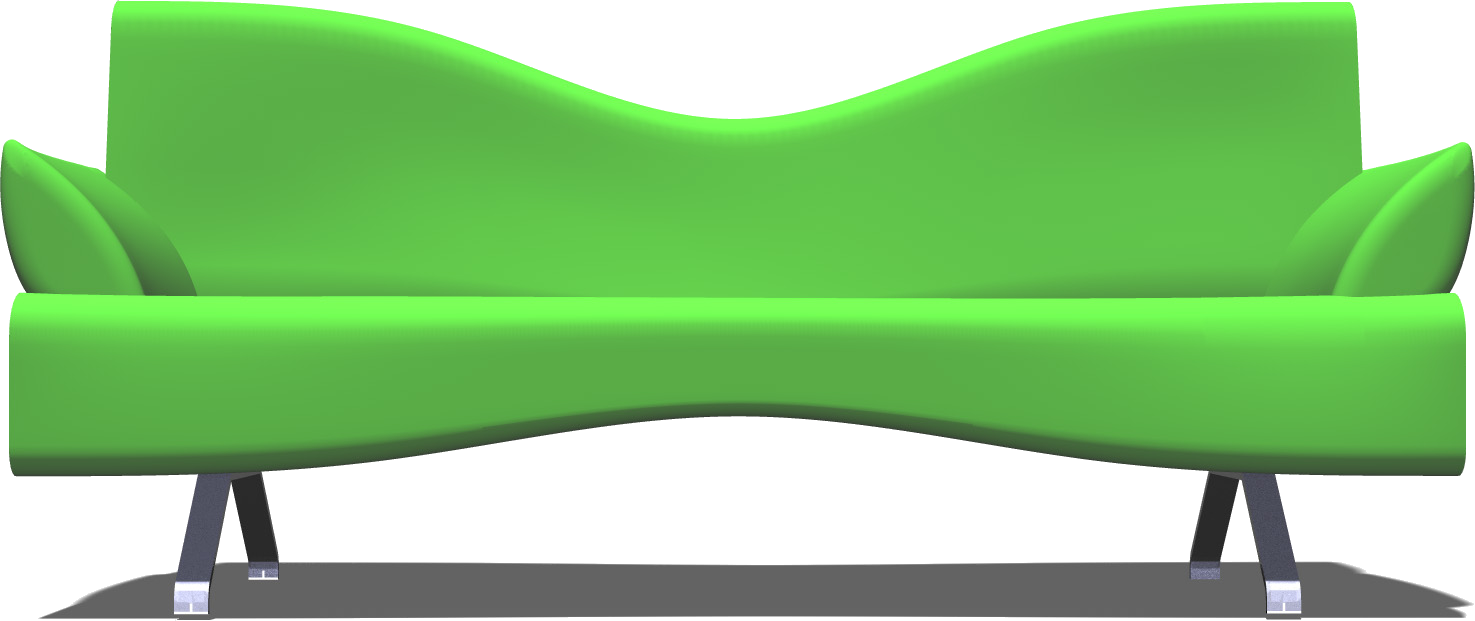
\includegraphics[width=.9\textwidth]{images/cosyverif.png}

  \smallskip

  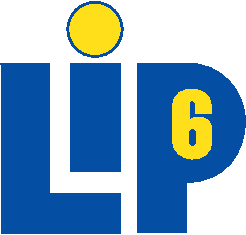
\includegraphics[height=5em]{images/lip6.pdf}~~~~~
  
\includegraphics[height=4em]{images/lipn.pdf}~~~~~
  
\includegraphics[height=5em]{images/lsv.pdf}

  \smallskip

  
\includegraphics[height=3em]{images/cnrs.png}
  
\includegraphics[height=3em]{images/inria.png}
  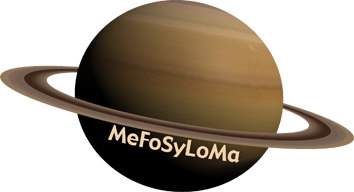
\includegraphics[height=3em]{images/mefosyloma.png}
  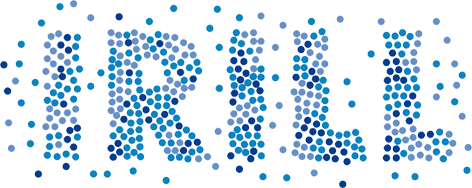
\includegraphics[height=3em]{images/irill.png}
  \end{center}  
\end{frame}

\begin{frame}
  \frametitle{\href{http://cosyverif.org}{CosyVerif} :
  un environnement de Modélisation \& Vérification}
  \begin{center}
  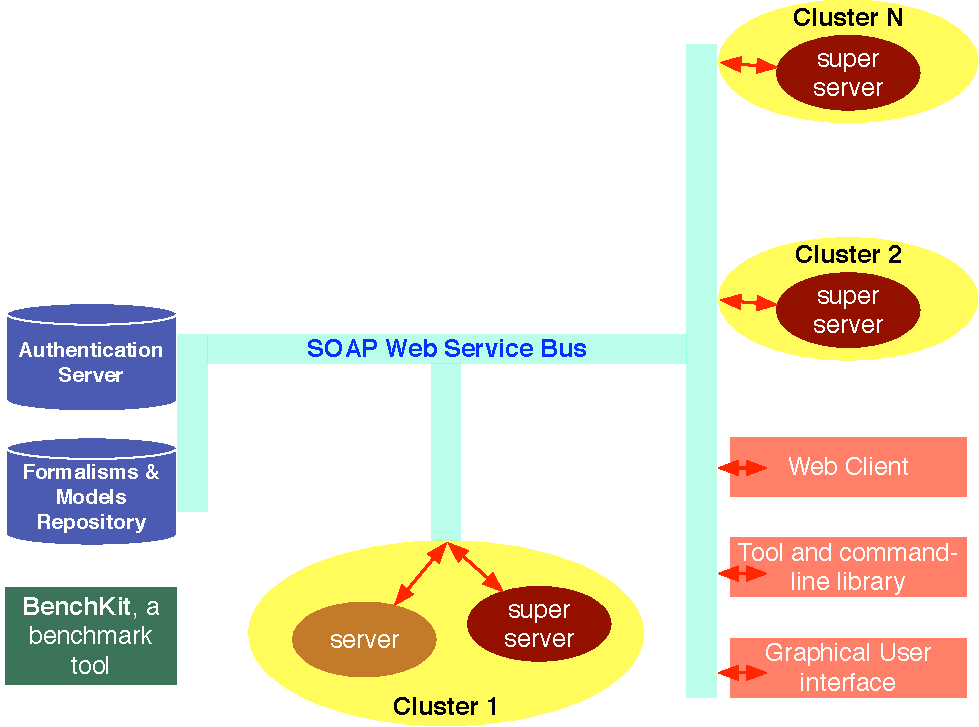
\includegraphics[height=7cm]{images/architecture.pdf}
  \end{center}
\end{frame}

\begin{frame}
  \frametitle{1. Circuit à sens unique}
  \begin{block}{Description}
  Deux trains circulent dans le même sens sur une voie formant une boucle.
  \end{block}

  \begin{itemize}
  \item Présentation en jeu
  \item Modélisation
  \item Quels problèmes sont envisagés ?
  \item Vérification
  \item Test en jeu
  \end{itemize}
\end{frame}

\begin{frame}
  \frametitle{2. Ajout de signaux de blocage}
  \begin{block}{Description}
  On divise la boucle en quatre sections avec des signaux.

  Un signal empêche le train de passer si un autre train se trouve dans la section suivante.
  \end{block}

  \begin{itemize}
  \item Présentation en jeu
  \item Modélisation
  \item Quels problèmes sont envisagés ?
  \item Vérification
  \item Test en jeu
  \end{itemize}
\end{frame}

\begin{frame}
  \frametitle{3. Économie de signaux de blocage}
  \begin{block}{Description}
  On réduit le nombre de signaux pour n'en garder que deux.
  \end{block}

  \begin{itemize}
  \item Présentation en jeu
  \item Modélisation
  \item Quels problèmes sont envisagés ?
  \item Vérification
  \item Test en jeu
  \end{itemize}
\end{frame}

\begin{frame}
  \frametitle{4. Circulation bidirectionnelle}
  \begin{block}{Description}
  Sans aucun signaux, on autorise deux trains à rouler en sens inverse.
  \end{block}

  \begin{itemize}
  \item Présentation en jeu
  \item Modélisation
  \item Quels problèmes sont envisagés ?
  \item Vérification
  \item Test en jeu
  \end{itemize}
\end{frame}

\begin{frame}
  \frametitle{5. Ajout de signaux de blocage}
  \begin{block}{Description}
  On ajoute quatre signaux de blocage.
  \end{block}

  \begin{itemize}
  \item Présentation en jeu
  \item Modélisation
  \item Quels problèmes sont envisagés ?
  \item Vérification
  \item Test en jeu
  \end{itemize}
\end{frame}

\begin{frame}
  \frametitle{6. Trains à la dérive}
  \begin{block}{Description}
  Deux trains peuvent se garer sur trois voies de garage.
  \end{block}

  \begin{itemize}
  \item Présentation en jeu
  \item Modélisation
  \item Quels problèmes sont envisagés ?
  \item Vérification
  \item Test en jeu
  \end{itemize}
\end{frame}

\begin{frame}
  \frametitle{7. Gare optimisée}
  \begin{block}{Description}
  Des trains circulent sur des voies à sens unique entre des gares
  un peu particulières.
  \end{block}

  \begin{itemize}
  \item Présentation en jeu
  \item Modélisation
  \item Quels problèmes sont envisagés ?
  \item Vérification
  \item Test en jeu
  \end{itemize}
\end{frame}

\begin{frame}
  \frametitle{8. \& 9.  Tronçon à une ou deux voies}
  \begin{block}{Description}
    Deux gare sont relié par une unique voie utilisez dans les deux
    sens. Deux train circule entre ces deux gares.
  \end{block}

  \begin{itemize}
  \item Présentation en jeu
  \item Modélisation
  \item Quel gain de temps avec deux voies?

  \end{itemize}
\end{frame}

\begin{frame}
  \frametitle{10. Croisement de trains}
  \begin{block}{Description}
  Deux trains doivent se croiser à une intersection (protégée par une barrière).
  Quel doit être le délai entre la détection du train et
  le signal de fermeture de la barrière ? 
  \end{block}

  \begin{itemize}
  \item Présentation en jeu
  \item Quels problèmes sont envisagés ?
  \item Modélisation
  \item Calcul du délai
  \end{itemize}
\end{frame}

\end{document}
